\documentclass[tikz,border=12pt]{standalone}
\usepackage{tikz}
\usetikzlibrary{positioning, arrows.meta, shapes.misc, fit, backgrounds, calc}

% Professional ACM/IEEE Academic Color Palette
\definecolor{acmPrimary}{RGB}{15, 60, 115}       % Deep Academic Blue
\definecolor{acmSecondary}{RGB}{35, 105, 165}   % Medium Steel Blue
\definecolor{acmAccent}{RGB}{60, 145, 205}      % Accent Blue
\definecolor{acmDarkGray}{RGB}{45, 55, 70}       % Dark Slate Text
\definecolor{acmLightBg}{RGB}{246, 248, 252}    % Box Light Shading
\definecolor{acmBoxBg}{RGB}{255, 255, 255}      % Card White Fill
\definecolor{acmGroupBg}{RGB}{236, 242, 249}    % Container Fill

\begin{document}

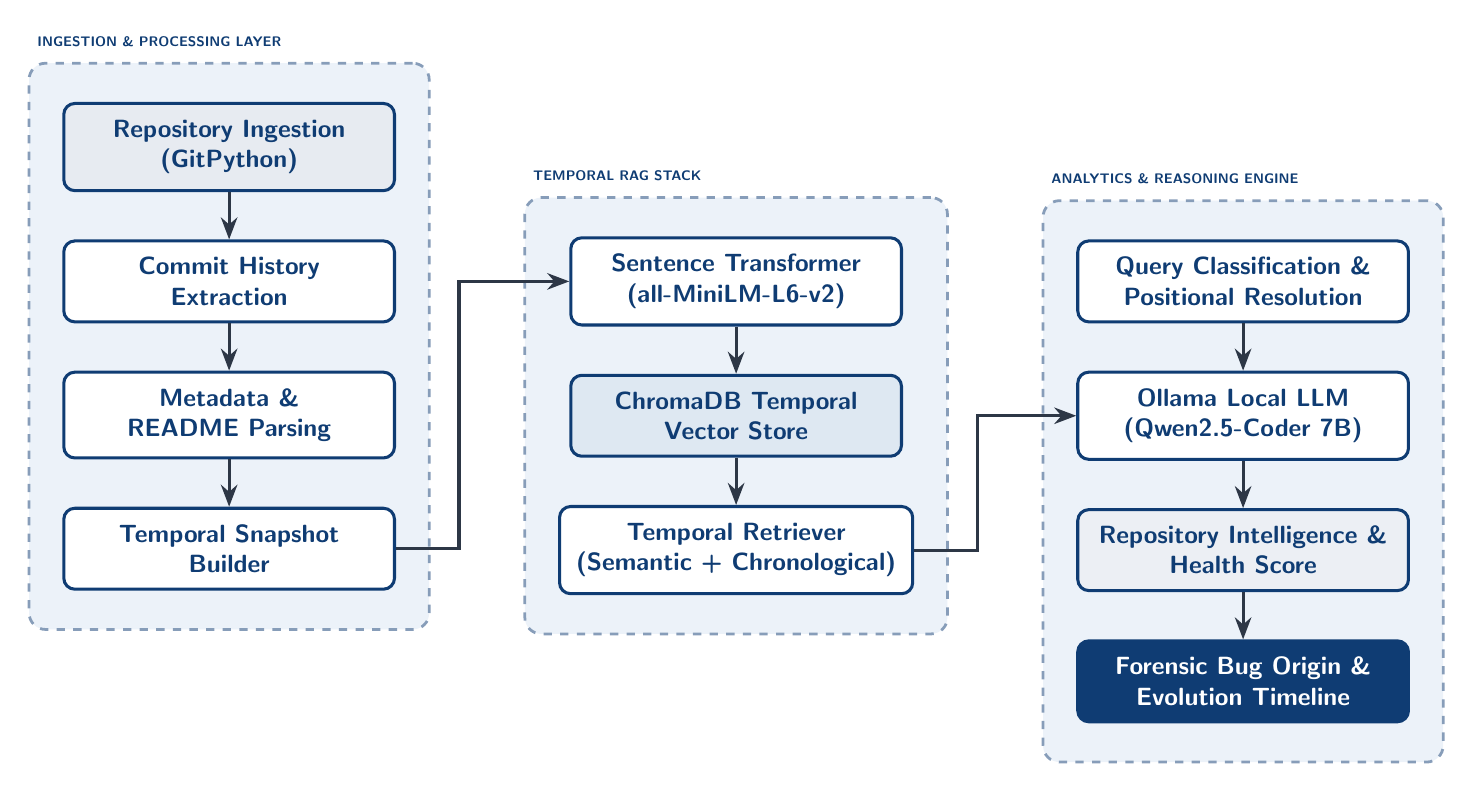
\begin{tikzpicture}[
    font=\sffamily\small,
    >=Stealth,
    node distance=0.65cm and 2.0cm,
    box/.style={
        draw=acmPrimary,
        fill=acmBoxBg,
        rectangle,
        rounded corners=4pt,
        line width=1.1pt,
        align=center,
        inner sep=6pt,
        minimum width=4.2cm,
        minimum height=0.95cm,
        font=\sffamily\small\bfseries\color{acmPrimary}
    },
    header/.style={
        font=\sffamily\tiny\bfseries,
        color=acmPrimary,
        align=center
    },
    arrow/.style={
        draw=acmDarkGray,
        ->,
        line width=1.1pt
    },
    container/.style={
        draw=acmPrimary!50,
        fill=acmGroupBg,
        rectangle,
        dashed,
        rounded corners=6pt,
        line width=1.0pt,
        inner ysep=14pt,
        inner xsep=12pt
    }
]

% 1. Ingestion Layer (Column 1)
\node[box, fill=acmPrimary!10] (ingest) {Repository Ingestion\\(GitPython)};
\node[box, below=0.6cm of ingest] (extract) {Commit History\\Extraction};
\node[box, below=0.6cm of extract] (parse) {Metadata \&\\README Parsing};
\node[box, below=0.6cm of parse] (snapshot) {Temporal Snapshot\\Builder};

\begin{scope}[on background layer]
    \node[container, fit=(ingest) (extract) (parse) (snapshot)] (ingest_group) {};
    \node[header, anchor=south west, yshift=2pt] at (ingest_group.north west) {INGESTION \& PROCESSING LAYER};
\end{scope}

\draw[arrow] (ingest) -- (extract);
\draw[arrow] (extract) -- (parse);
\draw[arrow] (parse) -- (snapshot);

% 2. Temporal RAG Stack (Column 2)
\node[box, right=2.2cm of extract] (embed) {Sentence Transformer\\(all-MiniLM-L6-v2)};
\node[box, fill=acmSecondary!15, below=0.6cm of embed] (chroma) {ChromaDB Temporal\\Vector Store};
\node[box, below=0.6cm of chroma] (retrieve) {Temporal Retriever\\(Semantic + Chronological)};

\begin{scope}[on background layer]
    \node[container, fit=(embed) (chroma) (retrieve)] (rag_group) {};
    \node[header, anchor=south west, yshift=2pt] at (rag_group.north west) {TEMPORAL RAG STACK};
\end{scope}

\draw[arrow] (snapshot.east) -- ++(0.8,0) |- (embed.west);
\draw[arrow] (embed) -- (chroma);
\draw[arrow] (chroma) -- (retrieve);

% 3. Analytics & Reasoning Engine (Column 3)
\node[box, right=2.2cm of chroma] (llm) {Ollama Local LLM\\(Qwen2.5-Coder 7B)};
\node[box, above=0.6cm of llm] (query) {Query Classification \&\\Positional Resolution};
\node[box, fill=acmPrimary!8, below=0.6cm of llm] (intel) {Repository Intelligence \&\\Health Score};
\node[box, fill=acmPrimary, text=white, below=0.6cm of intel] (bug) {Forensic Bug Origin \&\\Evolution Timeline};

\begin{scope}[on background layer]
    \node[container, fit=(query) (llm) (intel) (bug)] (reason_group) {};
    \node[header, anchor=south west, yshift=2pt] at (reason_group.north west) {ANALYTICS \& REASONING ENGINE};
\end{scope}

\draw[arrow] (query) -- (llm);
\draw[arrow] (retrieve.east) -- ++(0.8,0) |- (llm.west);
\draw[arrow] (llm) -- (intel);
\draw[arrow] (intel) -- (bug);

\end{tikzpicture}

\end{document}
